\chapter{毒理测试平台在线虫实验中的应用}
\section{引言}
	在本文的前两章,分别对毒理测试平台的软硬件做了详细的介绍。
	本章内容为本文的实验部分。为了展示本平台在毒理测试方面的应用优势,本章针对前文介绍的
	两款毒理测试芯片设计了两个实验。针对用于急性毒性实验的梯度微流控芯片,
	本文运用这款芯片研究了线性浓度梯度双氧水对线虫活性的影响,
	并将线虫身体摆动频率作为主要的监测指标。实验中视频数据的分析部分,通过使用第三章中介绍的
	线虫跟踪和特征提取算法完成,成功实现了线虫的跟踪和对体长、身体摆动频率特征的监测。
	与传统的基于96孔板上的线虫实验相比,无论是实验操作还是实验数据的分析都体现了本平台自动化、
	操作灵活、方便快捷、实验周期短等优势。
	针对第二款带侧向阀门的线虫培养芯片,本文设计了一个线虫进样实验,
	通过控制侧向阀门的压力来控制腔室入口通道的宽度。
	实验结果显示利用该芯片的侧向阀门可以很好地控制腔室中线虫进入。
\section{线虫的氧化急性应激实验}
	氧化应激(Oxidative Stress,OS)指生物体氧化与抗氧化作用的失衡,当生物体被内外环境中
	存在有害化合物刺激时,其体内所产生的活性氮自由基和活性氧自由基将会导致细胞或者组织发生生理和
	病理反应。过氧化氢($H_2O_2$)溶液作为一种强氧化剂经常被用于线虫的氧化应激实验中。本文
	将野生型N2秀丽隐杆线虫的L1期幼虫作为研究对象,通过本文前面介绍的软硬件平台,研究不同线性
	浓度梯度的双氧水溶液对L1期幼虫活性的影响。
\subsection{线虫的同步化}
	为了得到处于同一发育阶段的幼虫需要对线虫进行同步化处理,首先用经过高压灭菌的M9缓冲液将NGM平板上
	混合发育期的线虫冲洗到1.5ml的离心管中,离心后去掉上清液,加入碱裂解液(体积比为1:2的5N NaOH溶液和
	5\%NaClO溶液,现配),当线虫全被腐蚀时,液体将变得清澈。再经过离心处理,去掉上层碱裂解液加入M9
	缓冲液,离心洗涤1到2次。去掉上层缓冲液并用吸管将线虫卵接种到NGM平板上,至此便完成了同步化操作,等
	线虫卵孵化便得到同步化的个体。
\subsection{线性梯度稀释芯片的操作}
	图\ref{fig:chap5:chip}为梯度稀释芯片示意图,图\ref{fig:sysdevice}是实验硬件部分连接示意图。芯片上所有的阀门控制和进样控制均由Arduino单片机
	通过uln2803集成芯片控制多路电磁阀实现。在实验之前需要准备线虫溶液,
	将含有L1期幼虫的溶液离心去除上清液得到线虫浓缩液,
	然后再用移液枪加入0.25\%的琼脂糖溶液作为线虫助悬剂,至此便得到线虫溶液。芯片的实验操作按照以下步骤进行:
	\begin{figure}[!t]
	  \centering
	  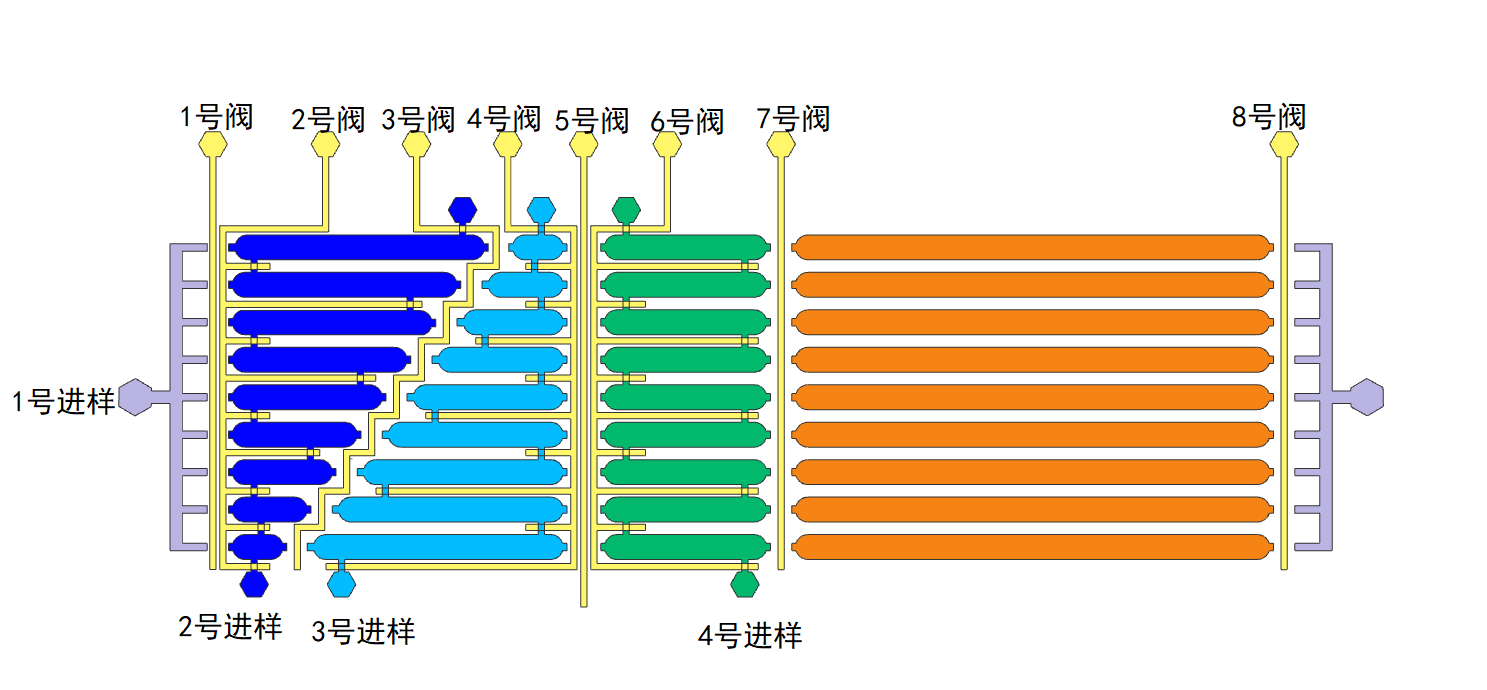
\includegraphics[width=14cm]{figure/chap5/chip.png}
	  \bicaption
		{梯度稀释芯片的示意图}
		{Schematic diagram of a gradient dilution chip}
	  \label{fig:chap5:chip}
	\end{figure}

	
	\begin{enumerate}[label={(\arabic*)},font={\color{black!50!black}\bfseries}]
	\item 首先打开6号阀门,采用压力进样的方式将线虫溶液从4号进样口打入第三列腔室。
	\item 打开4号阀门用压力进样的方式将M9缓冲液从3号进样口打入第二列腔室。
	\item 然后打开2号阀门用压力进样的方式将30mM的过氧化氢溶液从2号进样口打入第一列腔室。
	\item 然后关闭2号阀门、4号阀门和6号阀门,打开1号阀门、3号阀门、5号阀门和7号阀门。
	\item 在1进样口施加一个周期为250ms的气压,通过振荡的方式使前三列腔室中的液体充分混合均与。
	\item 最后通过进样口1将稀释好的线虫过氧化氢溶液打入第四列腔室。
	\item 用DigiRetina 16相机采集线虫在9个腔室中的运动视频。
	\end{enumerate}
	根据梯度稀释芯片各个腔室的加工尺寸,可以计算出混合后各腔室的过氧化氢溶液的浓度从最上面一排腔室至
	最下面一排腔室依次为:
	18mM、16mM、14mM、12mM、10mM、8mM、6mM、4mM和2mM。

	\begin{figure}[!t]
	  \centering
	  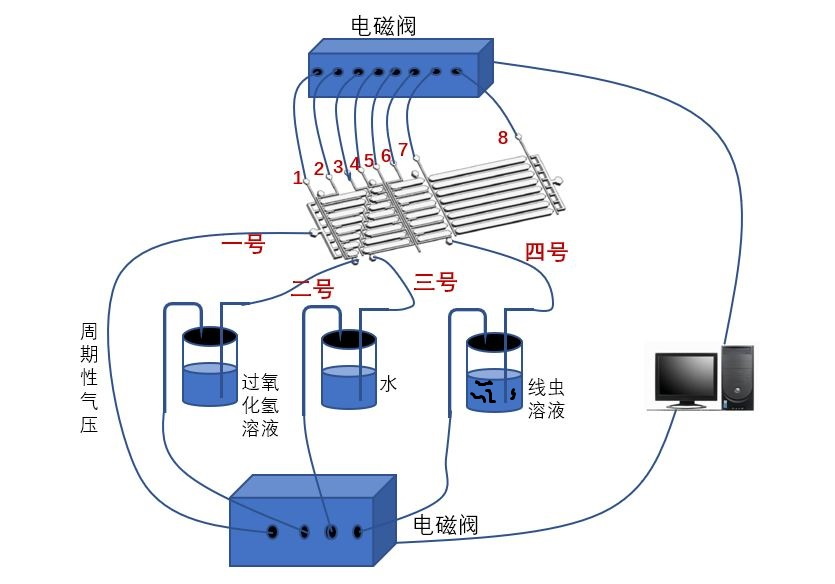
\includegraphics[width=11cm]{figure/chap5/hardware.jpg}
	  \bicaption
		{实验系统装置示意图}
		{Experimental system device schematic}
	  \label{fig:sysdevice}
	\end{figure}

\subsection{秀丽隐杆线虫急性氧化应激实验结果}
	实验视频数据的分析是通过本文前面提出的线虫轮廓分割、轮廓解析、轮廓跟踪及特征提取算法完成的,对每个腔室的
	视频数据进行分析并提取身体摆动频率、体长等特征,图\ref{fig:trackres}显示了梯度稀释
	芯片最下面一个腔室中线虫跟踪的结果。从图中可以看出腔室中有四只L1
	期的线虫且分别用不同的Track ID标识,每一帧图像中所有线虫的体长和身体
	弯曲角度都可以通过第三章介绍的算法计算,图中线虫体长的单位为单位像素距离,
	角度的单位为度。图\ref{fig:angle}显示的是Track ID为2和4的
	线虫其身体弯曲角随时间变化的摆动曲线,可以看出其身体弯曲角在$180^\circ C$左右
	振荡。通过对九个腔室中的线虫运动视频进行分析,可以得到不同时刻
	九个腔室中线虫的平均身体摆动频率的变化如图\ref{fig:res}所示。从图中可以看出随着过氧化氢溶
	液浓度的升高,线虫的身体摆动频率下降,且在同一过氧化氢溶液浓度下,线虫的身体摆动频率随着给药时
	间的增加而下降。为验证基于芯片平台的线虫实验的准确性,本文
	通过传统的稀释方法在96孔板上完成了相同线性浓度梯度的
	过氧化氢急性氧化应激实验,通过对各个时间点线虫平均身体摆动频率的统计,实验结果表明96孔板上的对照
	实验和基于梯度微流控芯片的线虫实验结果一致。但与之相比,本文提出的软硬件平台
	在试剂消耗、自动化程度和实验数据统计分析等上面都体现了较大的优势。
	\begin{figure}[H]
	  \centering
	  \includegraphics[width=14cm]{figure/chap5/trackres1.jpg}
	  \bicaption
		{梯度稀释芯片中线虫的跟踪结果}
		{Tracking results of C.elegans in a gradient dilution chip}
	  \label{fig:trackres}
	\end{figure}
	
	 \begin{figure}[h]
	  \centering
	  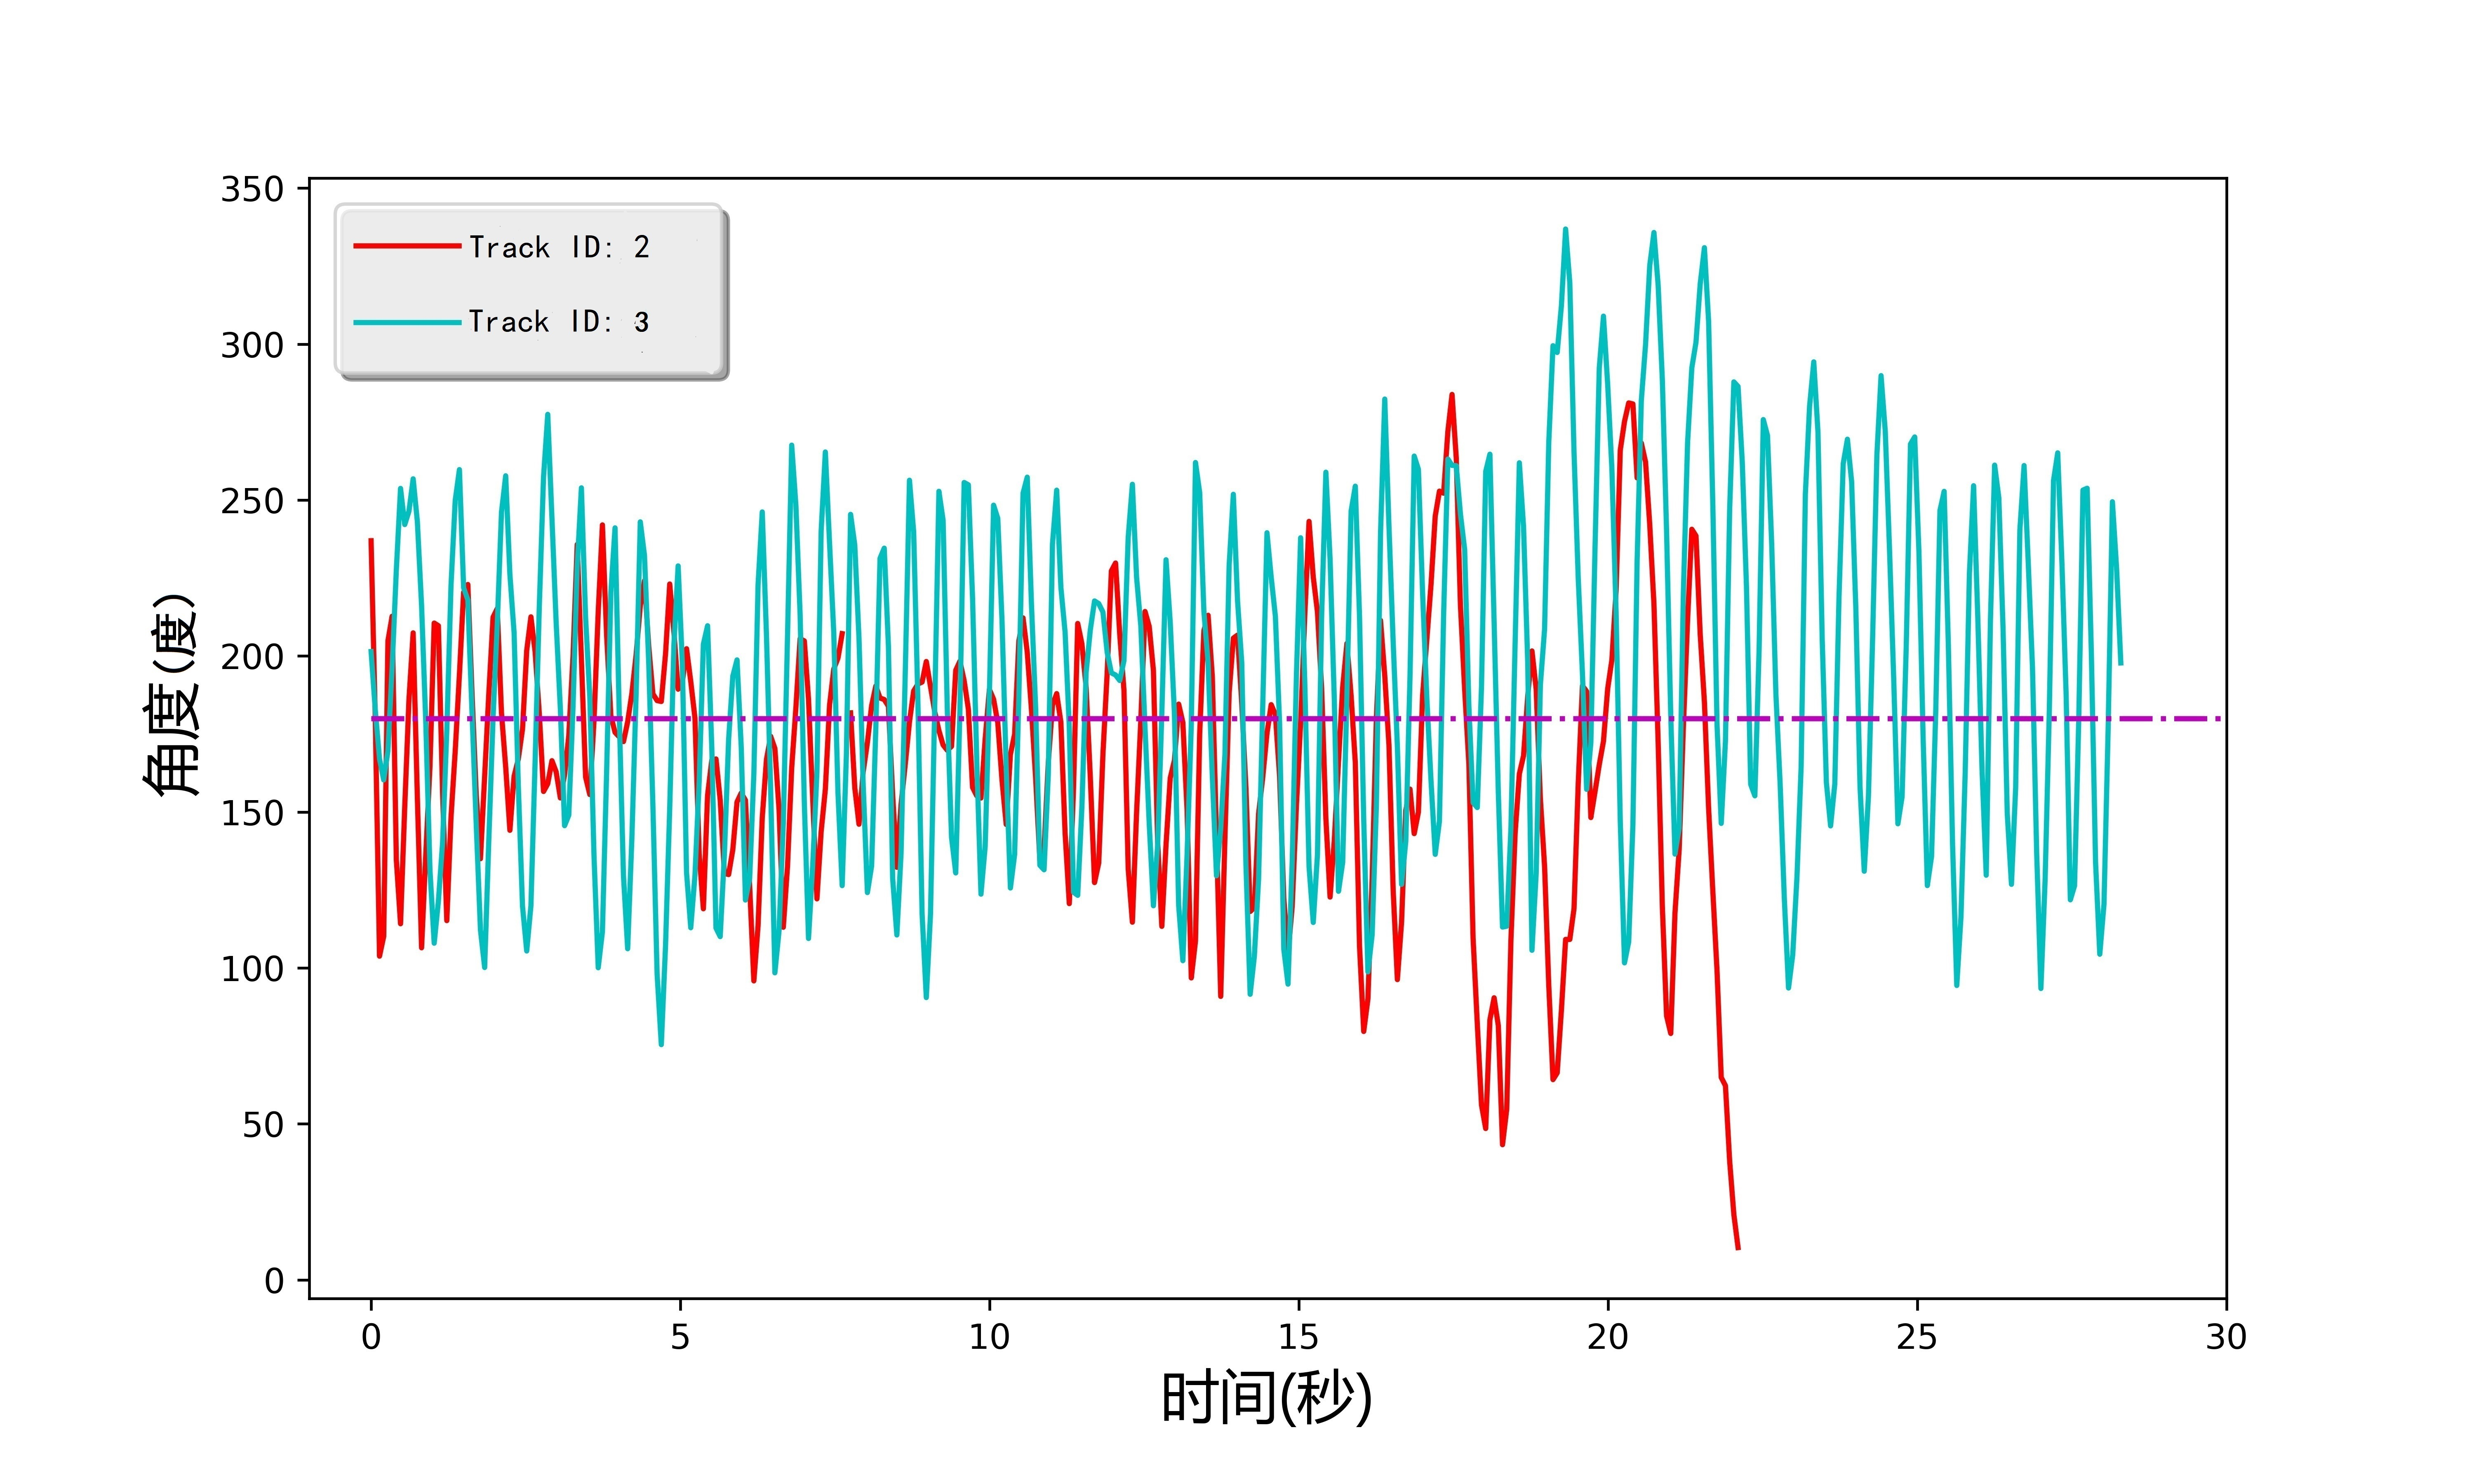
\includegraphics[width=14cm]{figure/chap5/angle.jpg}
	  \bicaption
		{线虫弯曲角度的变化}
		{Change in the bending angle of C.elegans}
	  \label{fig:angle}
	\end{figure}
	\begin{figure}[!h]
	  \centering
	  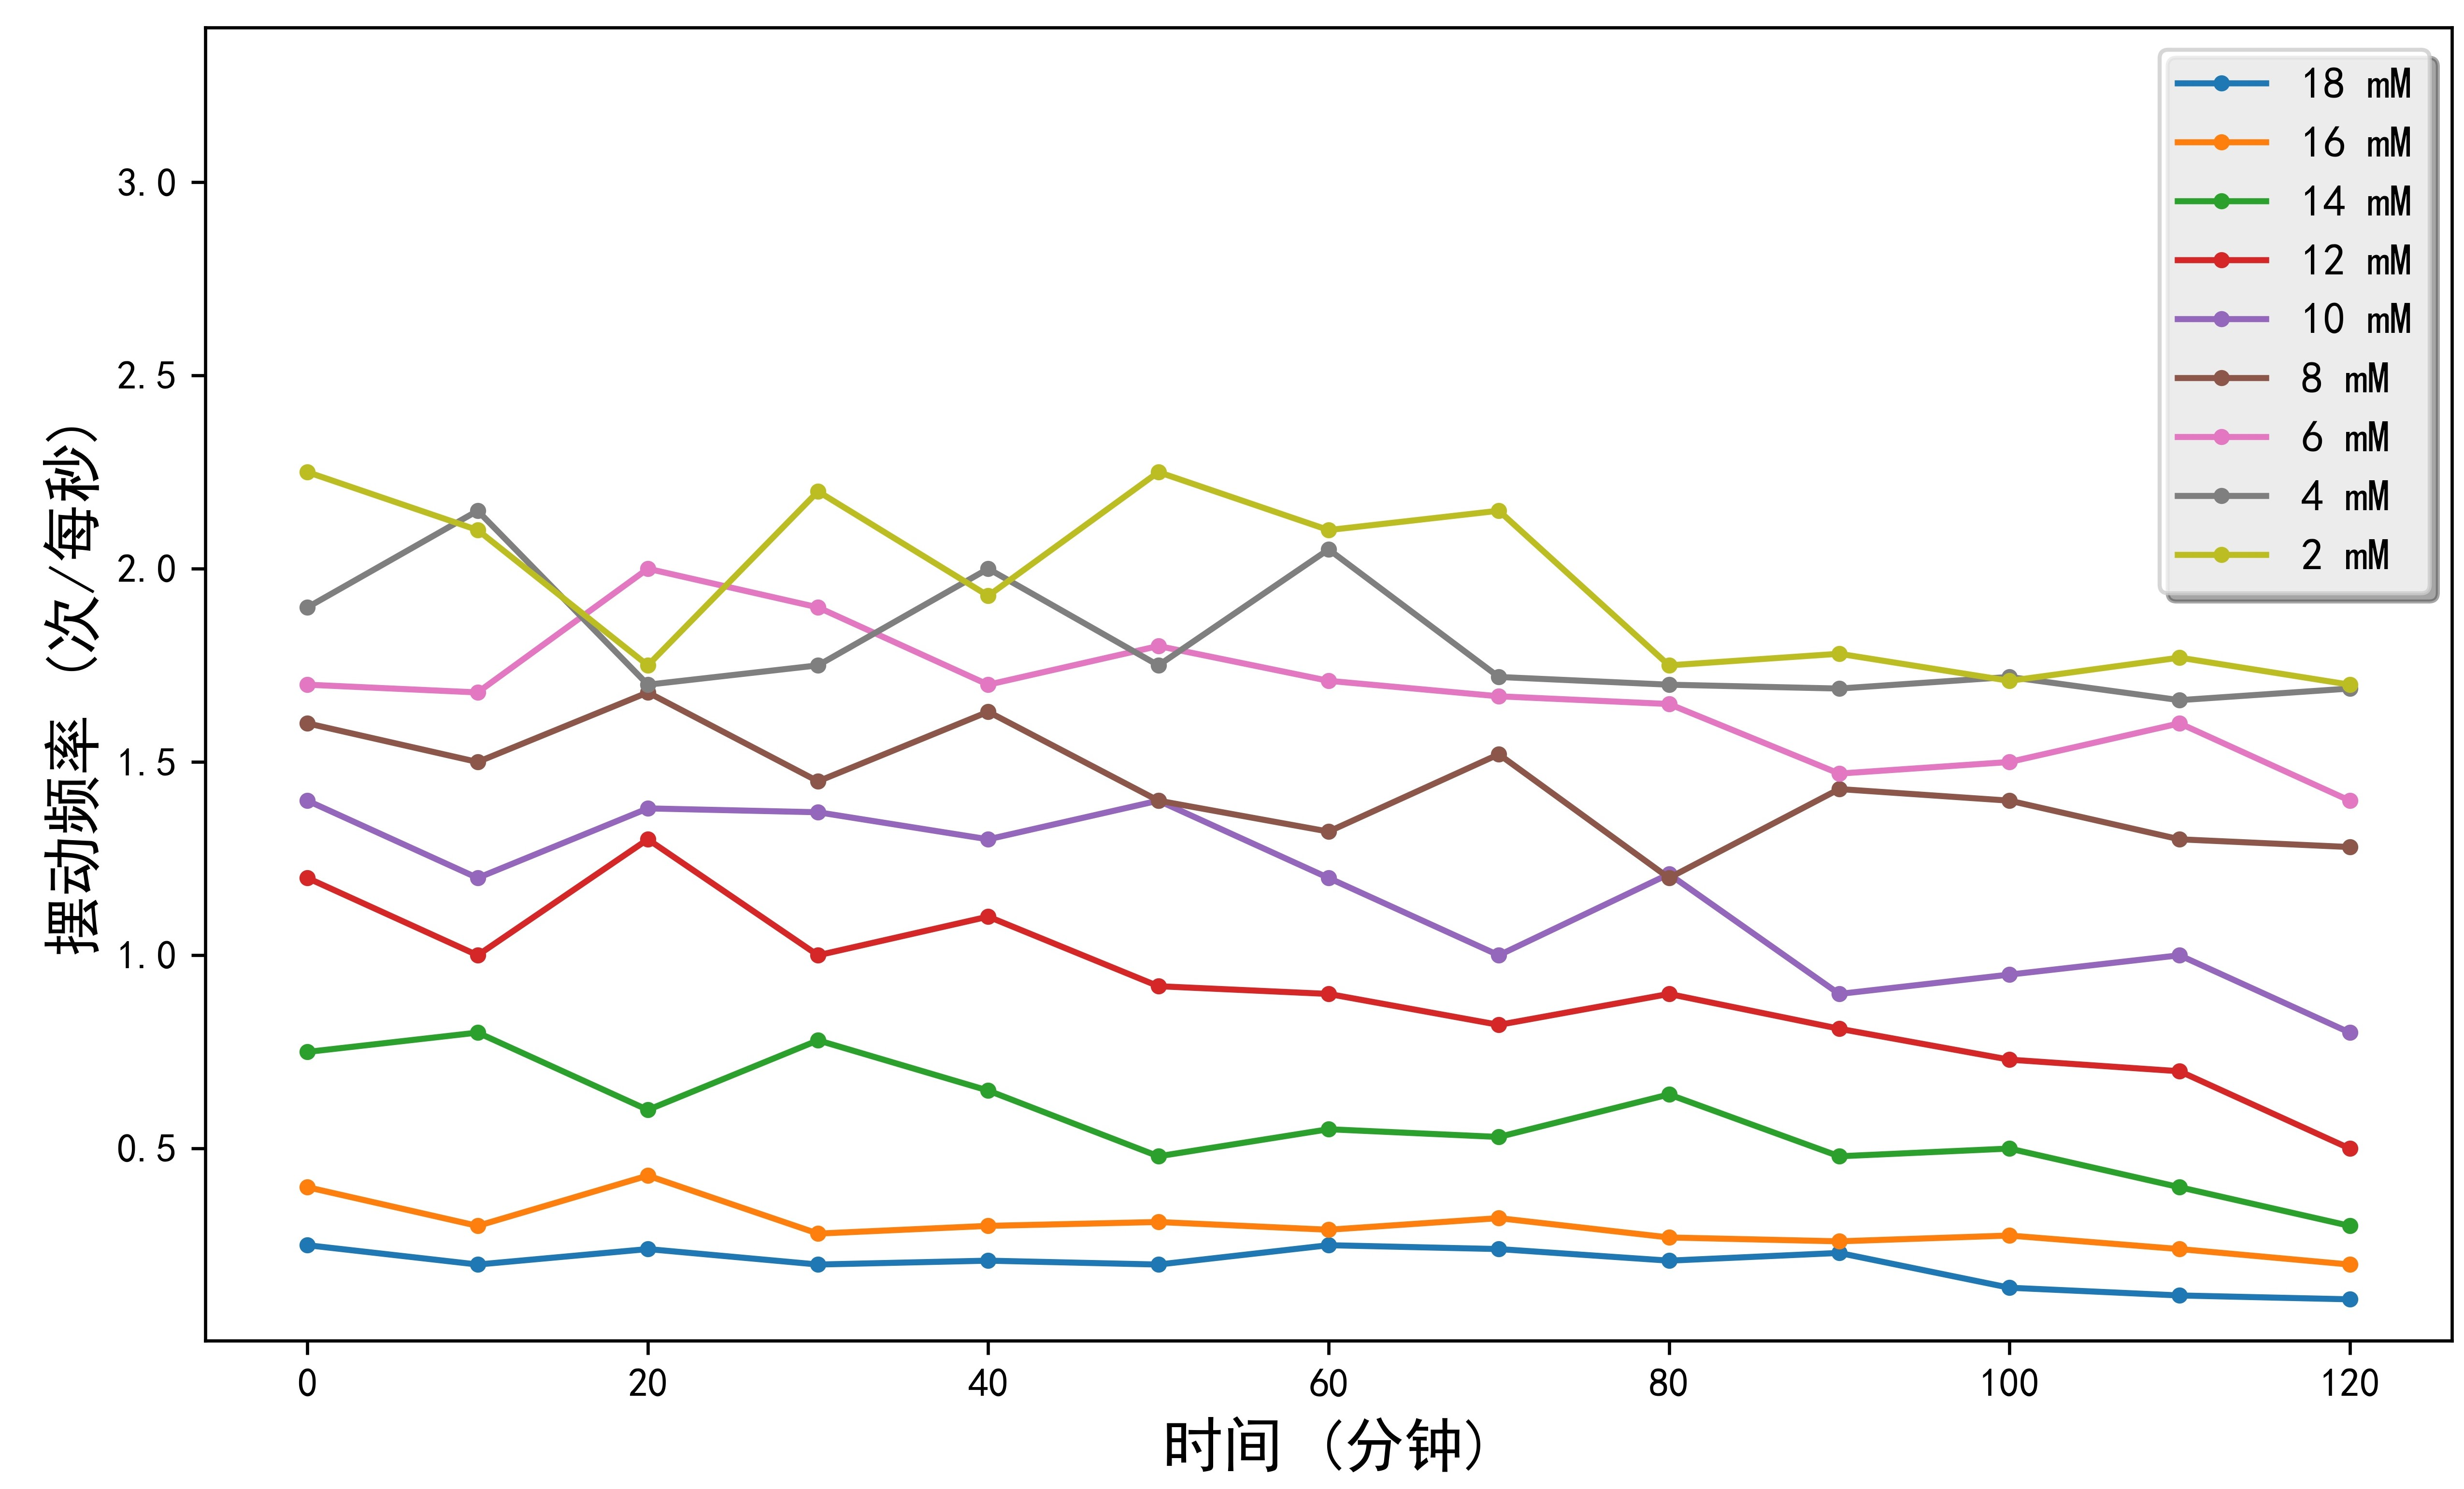
\includegraphics[width=13cm]{figure/chap5/res.jpg}
	  \bicaption
		{各腔室中线虫平均摆动频率随时间的变化}
		{The average swing frequency of C.elegans in each chamber changes with time}
	  \label{fig:res}
	\end{figure}
	
\section{线虫进样实验}
	在线虫相关毒理实验中,经常需要控制线虫进样的数量。腔室中线虫密度太高既不利于
	实验观察也给线虫的自动化图像分析带来很大困难。为此,本文设计了一款带侧向阀门的
	可以进行线虫长期培养的单层毒理芯片,
	片上两个侧向阀门分别控制线虫腔室的入口通道和出口通道的宽度。
	当需要向腔室中注入线虫时,将腔室进口通道的控制阀门打开,
	腔室出口通道的控制阀门关闭;当需要将线虫排出腔室中时,将腔室进口通道的控制阀门关闭
	,腔室出口通道的控制阀门打开;当需要保持腔室中线虫数量恒定时,
	将两个控制阀门全部关闭。图\ref{fig:chap5:worms}是线虫进样的过程图。在图\ref{fig:chap5:worms}a中线虫
	腔室的进入通道没有线虫,在图\ref{fig:chap5:worms}b中,由于向阀门施加气压后管道
	变窄,线虫被限制在管道中无法进入腔室。实验结果显示,侧向阀门的设计可以较好的
	控制线虫的进入。由于这款芯片设计了一个食物供应的通道
	,以及可以将腔室中的代谢废物和虫卵排出的侧面通道。该芯片可以对同一代的线虫进行长期
	培养观察,并监测其生理特征的变化,适用于线虫的慢性毒性实验。
	图\ref{fig:chap5:tracking2}表示对线虫培养腔室中线虫的跟踪结果。
	在实际应用中,该款芯片还可以当作辅助芯片配合其他线虫芯
	片使用。如需要控制一个腔室中线虫的数量时,可以先利用这款芯片缓冲
	到预定数量的线虫。然后再将这款芯片与目标芯片级联在一起,通过操纵阀门将
	线虫打入到目标腔室中,其作用相当于一个缓冲器的作用。
	\begin{figure}[!h]
	  \centering
	  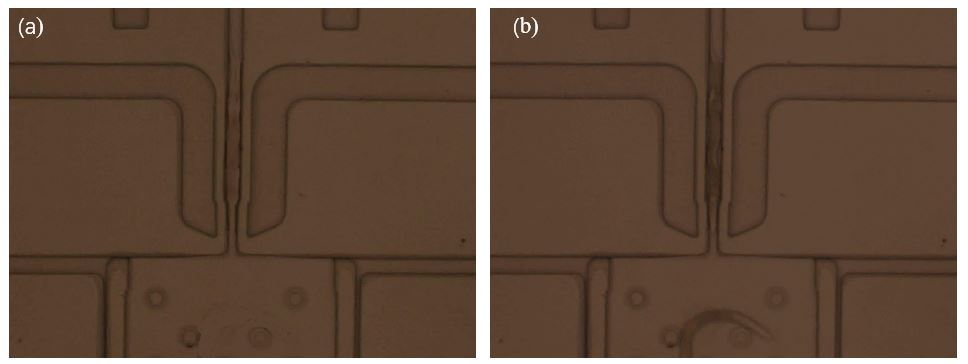
\includegraphics[width=15cm]{figure/chap5/valve.jpg}
	  \bicaption
		{线虫进样实验结果}
		{Experimental results of Caenorhabditis elegans injection}
	  \label{fig:chap5:worms}
	\end{figure}
	
	\begin{figure}[!h]
	  \centering
	  \includegraphics[width=13cm]{figure/chap5/trackres2.jpg}
	  \bicaption
		{线虫培养芯片中线虫的跟踪结果}
		{Tracking results of C.elegans in culture chips}
	  \label{fig:chap5:tracking2}
	\end{figure}
\newpage
\section{本章小结}
	本章为本文的实验部分,包含线虫急性氧化应激实验和线虫的进样实验。
	线虫的氧化应激实验主要研究了线性浓度梯度双氧水对线虫摆动频率的影响。
	在实验准备部分,介绍了线虫同步化的操作方法。在实验操作方面,
	介绍了线性梯度稀释芯片的操作步骤流程。在线虫摆动频率的监测方面
	,通过运用第三章介绍的线虫视频特征提取算法,分析了在给药两小时的过程
	中线虫摆动频率的变化。实验结果显示线虫的摆动频率随着过氧化氢溶液浓度
	的升高而下降,在同一浓度下线虫的摆动频率随着时间的延长也会下降。实验结
	果表明与96孔板上的对照实验结果一致,但与之相比,体现了本平台在自动化梯
	度稀释、试剂消耗、实验自动化和自动化特征提取方面均有很好的应用优势。针对
	第二章提出的用于慢性毒性实验的线虫培养芯片,本章设计了一个线虫进样实验,发现通过控制两个
	侧向阀门,该芯片可以很好的控制腔室中线虫的数量。未来可以利用这款芯片研究慢性毒物对线虫的
	长期影响。